\section{TINJAUAN PUSTAKA}

\subsection{\emph{Socially Assistive Robots}}

\begin{figure} [ht] \centering
  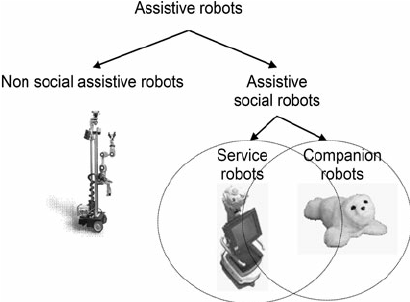
\includegraphics[scale=0.50]{gambar/robots-category.png}
  \caption{Pengategorian \emph{assistive robots} menurut Heerink et al. \citep{Heerink2010}}
  \label{fig:RobotsCategory}
\end{figure}

\emph{Socially assistive robots} (SARs) merupakan adaptasi dari \emph{assistive technology} yang meliputi keseluruhan sistem robotika yang mampu memberikan bantuan kepada pengguna dalam bentuk interaksi sosial \citep{Seifer2005}. Heerink et al. \citep{Heerink2010} mengategorikan riset terhadap SARs menjadi dua kategori berbeda seperti pada Gambar \ref{fig:RobotsCategory}.
Kategori pertama mencakup \emph{service robots} yang menawarkan bantuan fisik dan kognitif dan melakukan tugas sebagai pelayan, sedangkan kategori kedua mencakup \emph{companion robot} yang merupakan robot berjenis pendamping sebagai sahabat dan media untuk terapi.
Lebih lanjut Rich et al. \citep{Rich2009} menjelaskan SARs mampu memberikan bantuan kepada pengguna dalam berbagai tingkatan seperti:
(a) mendukung kemampuan fungsional dan kognitif pengguna;
(b) menawarkan pengguna kesempatan untuk meningkatkan partisipasi sosial dan kesehatan psikologis;
(c) menyediakan pemantauan jarak jauh dan berkelanjutan atas status kesehatan pengguna;
dan (d) membina pengguna untuk memfasilitasi promosi perilaku sehat dan pencapaian tujuan yang berhubungan dengan kesehatan.

\subsection{Robot Operating System 2 (ROS 2)}

Robot Operating System (ROS) \citep{Quigley2009} merupakan kumpulan dari libraries, drivers, dan tools yang mempermudah pengembangan sistem pada robot.
ROS memiliki command tool seperti Linux, sistem komunikasi antar proses, dan berbagai macam packages yang berhubungan dengan pengembangan sistem pada robot.
Proses yang dieksekusi pada ROS disebut sebagai Node, komunikasi antar proses yang dimiliki menggunakan model \emph{publish/subscribe}, dan data komunikasi yang dikirimkan disebut sebagai Topic.
Suatu proses Publisher mampu mengirimkan satu maupun lebih Topic, kemudian proses-proses lain yang melakukan subscribe pada suatu Topic bisa memperoleh isi dari Topic tersebut.
Selain itu ada juga Sevice yang memiliki fungsi seperti Topic, hanya saja dilakukan secara dua arah.
Service ini bekerja menggunakan model \emph{client/server} dimana Service Client akan mengirimkan data permintaan dalam bentuk Request dan kemudian Service Server akan mengirimkan data balasan dalam bentuk Response.

Generasi kedua dari Robot Operating System, ROS 2, merupakan kelanjutan dari ROS yang mengusung reliabilitas dan performa untuk penggunaan \emph{real-time} sembari masih mendukung keunggulan yang dimiliki oleh ROS sebelumnya \citep{Maruyama2016}.
Untuk memenuhi kebutuhan reliabilitas dan performa untuk penggunaan real-time tersebut, ROS 2 menggunakan \emph{Data Distribution Service} (DDS) \citep{Castellote2003} \citep{Schlesselman2004}, standar industri untuk sistem komunikasi real-time dan \emph{end-to-end middleware}, yang menggantikan sistem komunikasi antar proses yang dimiliki ROS sebelumnya.

\subsection{Gazebo}

Gazebo \citep{Koenig2004} merupakan bagian dari Player Project \citep{Gerkey2003} yang memungkinkan sebuah simulasi robot dan aplikasi sensor bekerja di lingkungan simulasi indoor maupun outdoor tiga dimensi.
Gazebo memiliki arsitektur \emph{client/server} dan model \emph{publish/subscribe} untuk sistem komunikasi antar prosesnya.
Setiap objek simulasi di Gazebo dapat diasosiasikan dalam satu maupun lebih kontroler yang akan memproses perintah untuk mengatur dan menentukan keadaan dari suatu objek.
Data yang dihasilkan oleh suatu kontroler akan dikirim ke \emph{shared memory} menggunakan Gazebo interfaces (ifaces).
Nantinya ifaces dari proses-proses lain dapat membaca data tersebut pada shared memory, sehingga memungkinkan komunikasi antar proses antara program yang mengontrol robot dan Gazebo, terlepas dari bahasa pemrograman yang digunakan.
